\begin{IEEEbiography}[{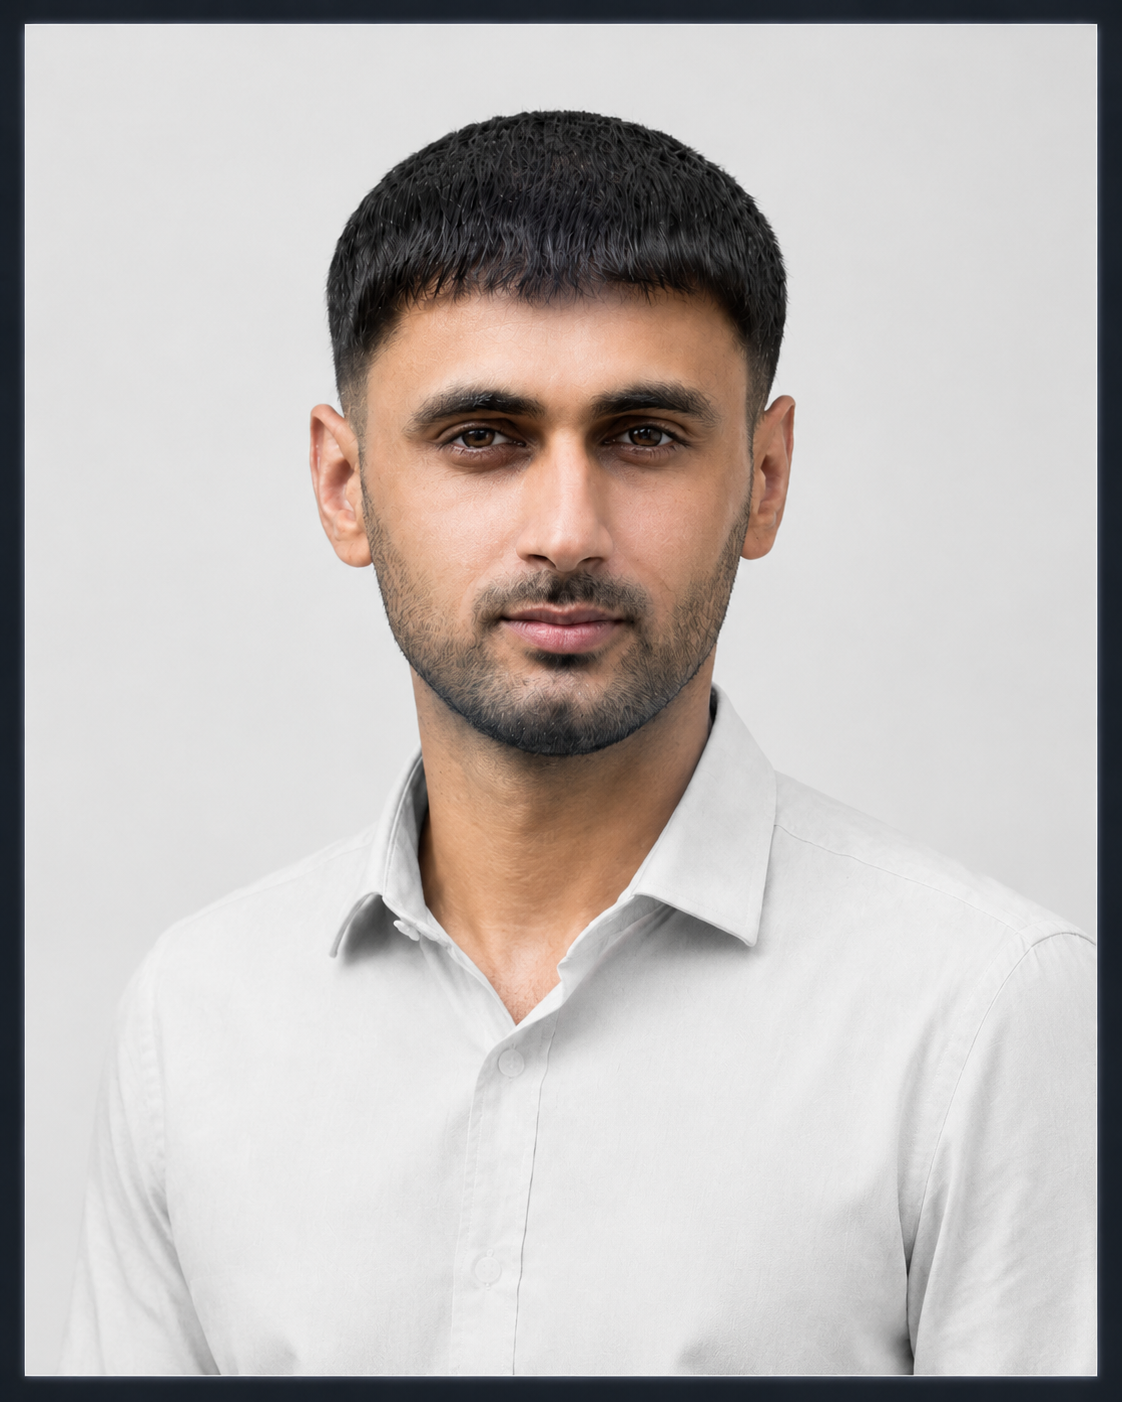
\includegraphics[width=1in,height=1.25in,clip,keepaspectratio]{figures/hasnain.png}}]{Hasnain Haider}
is pursuing the B.Sc. degree in Computer Science at Albukhary International University, Alor Setar, Kedah, Malaysia, under a fully funded international scholarship. His research interests include machine learning, interpretable artificial intelligence, financial fraud detection, computer vision, natural language processing, and real-world AI deployment. His current work focuses on leakage-controlled fraud-detection evaluation and interpretable decision-support systems.
\end{IEEEbiography}

\begin{IEEEbiography}[{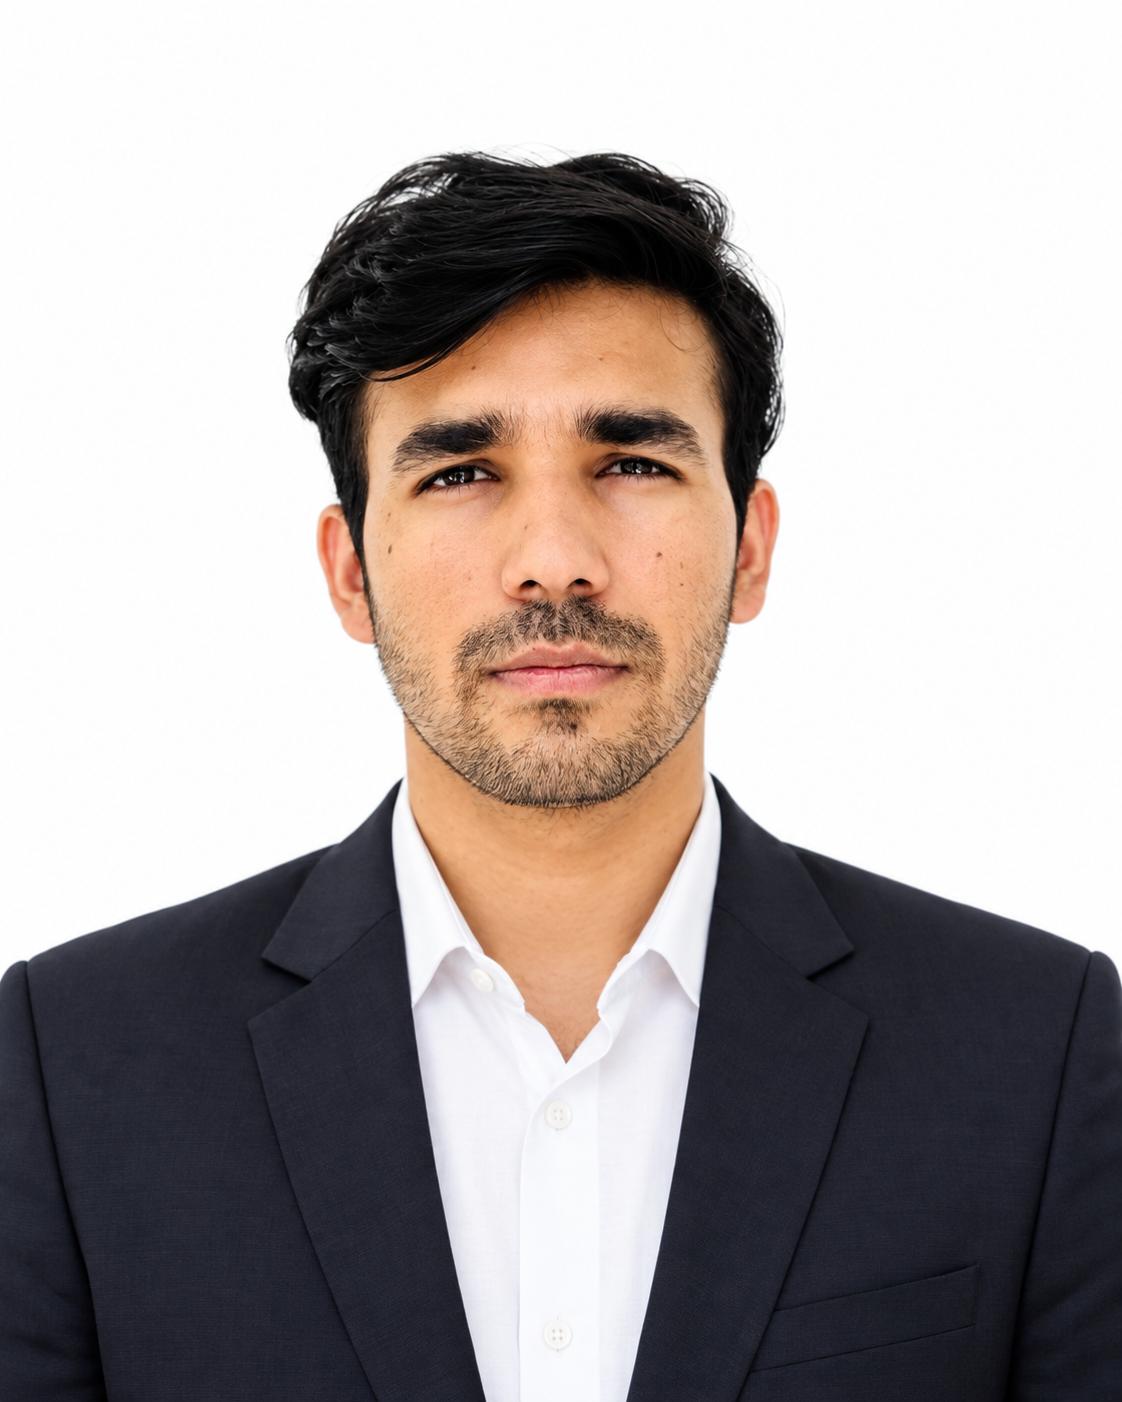
\includegraphics[width=1in,height=1.25in,clip,keepaspectratio]{figures/waseem.png}}]{Waseem Mushtaq}
is pursuing the B.Sc. degree in Computer Science at Albukhary International University, Alor Setar, Kedah, Malaysia, under a fully funded international scholarship. His research interests include machine learning, artificial intelligence, applied data science, and real-world AI systems. His recent work includes applied machine-learning projects and robust evaluation of financial fraud-detection models.
\end{IEEEbiography}

\begin{IEEEbiography}[{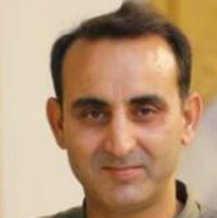
\includegraphics[width=1in,height=1.25in,clip,keepaspectratio]{figures/qaiser.png}}]{Qaiser Abbas}
received the M.S. degree in Computer Science from the National University of Computer and Emerging Sciences, Lahore, Pakistan, in 2010 and completed doctoral studies in Natural Language Processing and Computational Linguistics at the University of Konstanz, Germany, in 2014. He is currently with the Islamic University of Madinah, Madinah, Saudi Arabia. His research covers natural language processing, computational linguistics, machine learning, deep learning, mathematical modelling, and information retrieval. His ORCID is 0000-0003-1870-0884.
\end{IEEEbiography}

\begin{IEEEbiography}[{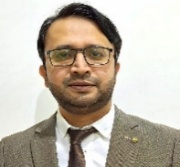
\includegraphics[width=1in,height=1.25in,clip,keepaspectratio]{figures/adnan.jpeg}}]{Adnan Nadeem Al Hassan}
(Senior Member, IEEE) received the Ph.D. degree from the University of Surrey, U.K., in 2011. He is a Full Professor and Head of the Department of Computer Science at the Islamic University of Madinah, Madinah, Saudi Arabia.
His work addresses real-world problems using the Internet of Things, advanced imaging, and artificial intelligence in smart cities, healthcare, agriculture, and security. His profile is available at \url{https://adnan-nadeem.com/}.
\end{IEEEbiography}

\begin{IEEEbiography}[{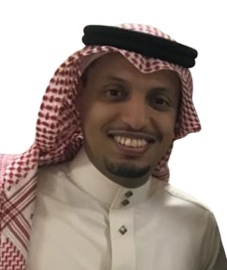
\includegraphics[width=1in,height=1.25in,clip,keepaspectratio]{figures/abdullah.jpeg}}]{Abdullah Alshanqiti}
received the Ph.D. degree in Computer Science from the University of Leicester, U.K. He is currently with the Faculty of Computer and Information Systems, Islamic University of Madinah, Madinah, Saudi Arabia.
His research interests include artificial intelligence, software engineering, model-driven engineering, responsible AI, federated machine learning, quantum machine learning, knowledge transfer, and image and language understanding.
\end{IEEEbiography}

\begin{IEEEbiography}[{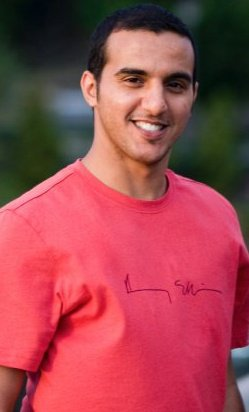
\includegraphics[width=1in,height=1.25in,clip,keepaspectratio]{figures/sami.jpeg}}]{Sami Albouq}
received the Bachelor's, Master's, and Doctoral degrees in Computer Science in 2009, 2011, and 2018, respectively. He is an Associate Professor with the Faculty of Computer and Information Systems, Islamic University of Madinah, Madinah 42351, Saudi Arabia.
His research interests include system security engineering, complex information technology systems, and quantum key distribution systems. His ORCID is 0009-0007-0955-544X.
\end{IEEEbiography}
